\chapter*{Week 1: Introduction}
\addcontentsline{toc}{chapter}{Week 1: Introduction}
\setcounter{chapter}{1}
\setcounter{section}{0}

\begin{abstract}
This week will cover:
\begin{enumerate}
    \item Learn how to compile and run a program in C++
    \item Learn a few basic variables
    \begin{itemize}
        \item Integers
        \item Floats
        \item Doubles
    \end{itemize}
    \item Terminal Input/Output
    \item How to write Pseudocode
\end{enumerate}
    
\end{abstract}

\section{Background}
This week will be an introduction to a variety of foundational material for computer science. You will need to learn how to navigate the required software, basic variables, user input, and algorithms/pseudocode. 

\subsection{Navigating Terminals and Compiling Code}
In Visual Studio Code, you can open an integrated terminal, which initially starts at the bottom of your workspace. But what is a terminal?

A \textbf{terminal} is an \textbf{interface} to your computer which allows you to execute any task on the computer directly through \textbf{commands}, without the use of a graphical user interface or GUI (like the file explorers on your system that you use to navigate to folders, create files etc). This allows you to directly execute tasks, which is often quicker than using the GUI.

VS Code has a built in terminal that you can open and use to interact with your computer's files and any code you write. To access this terminal, you will need to open VS Code. It may look like this the first time you open it:

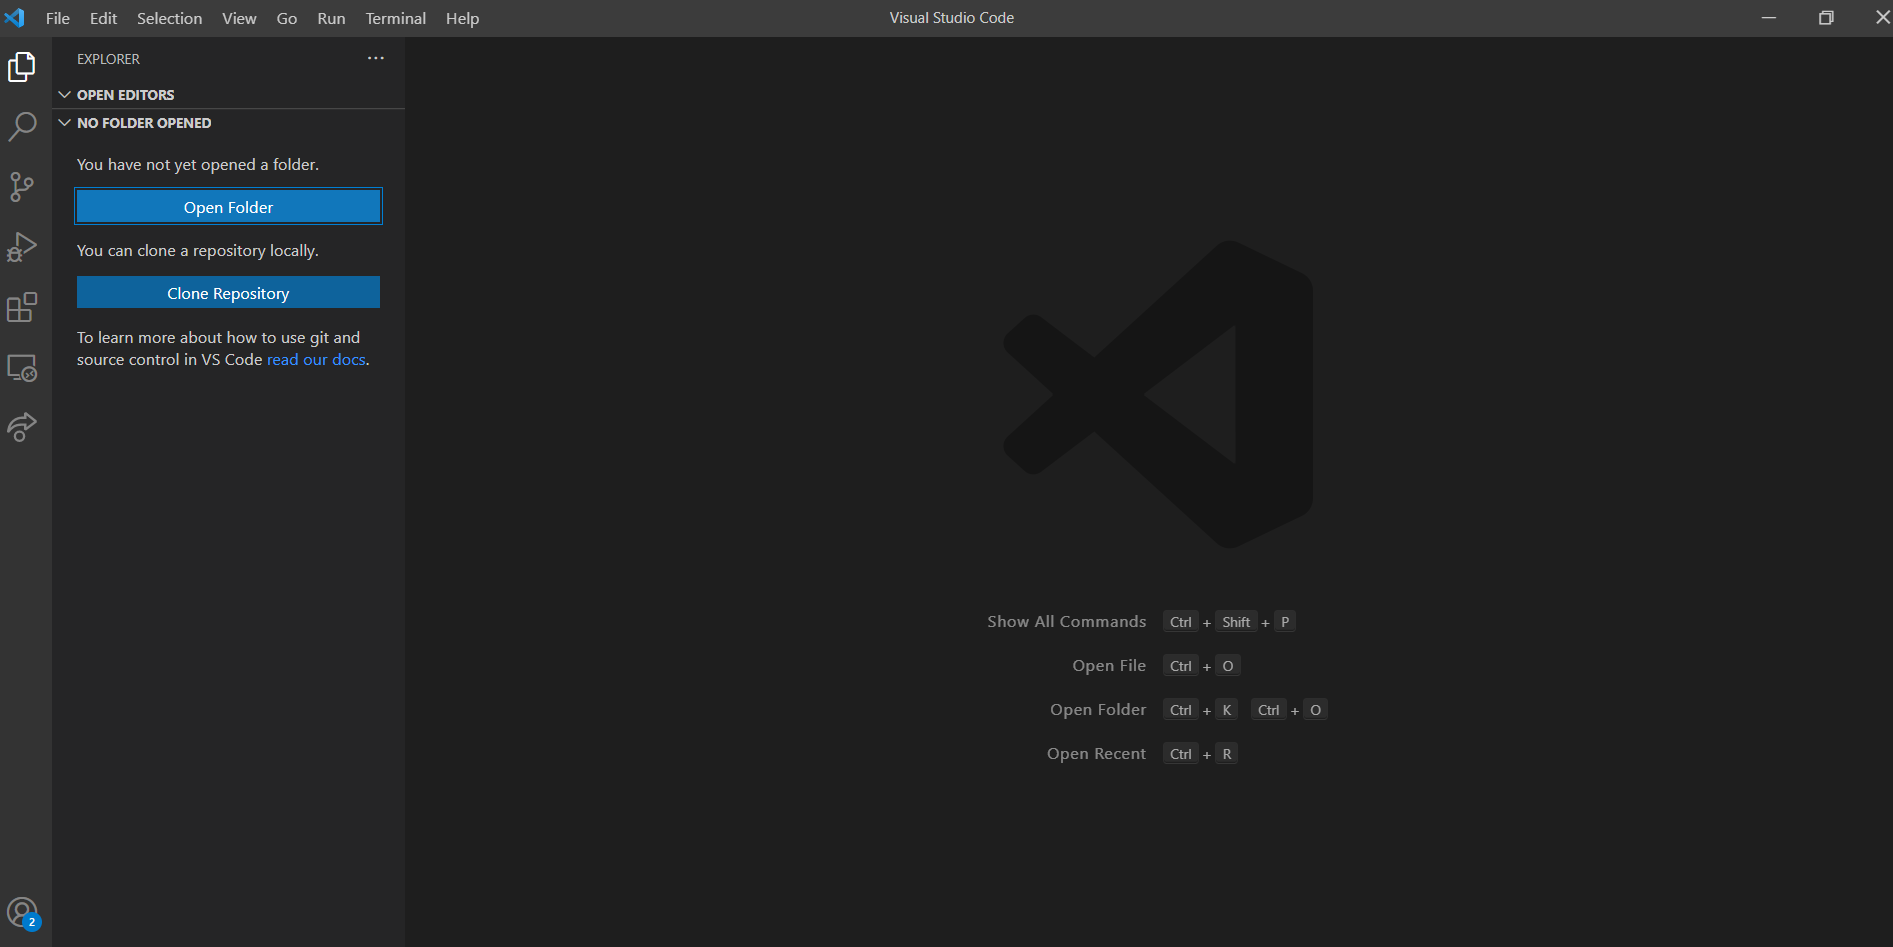
\includegraphics[width=\textwidth]{images/learn_terminal_1.png}

If you have not opened any folders yet in VS Code, you will need to start by opening one. You can do this by clicking ``Open Folder" and navigating to whichever folder you would like to use. I would encourage you to make a new folder called ``CSCI\_1300" to keep all of your course materials organized. 

Once you have a folder open, you can open a terminal. To open the Terminal tab, go to the menu bar, locate Terminal and click on it. Select ``New Terminal" to open a new terminal. A terminal looks like a dark screen when you open it and will open below the main window.

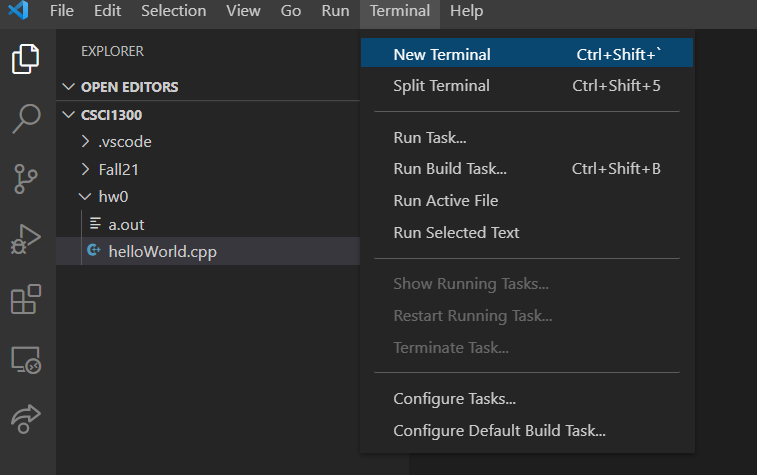
\includegraphics[width=\textwidth]{images/learn_terminal_3.png}

The new screen should look something like this: 

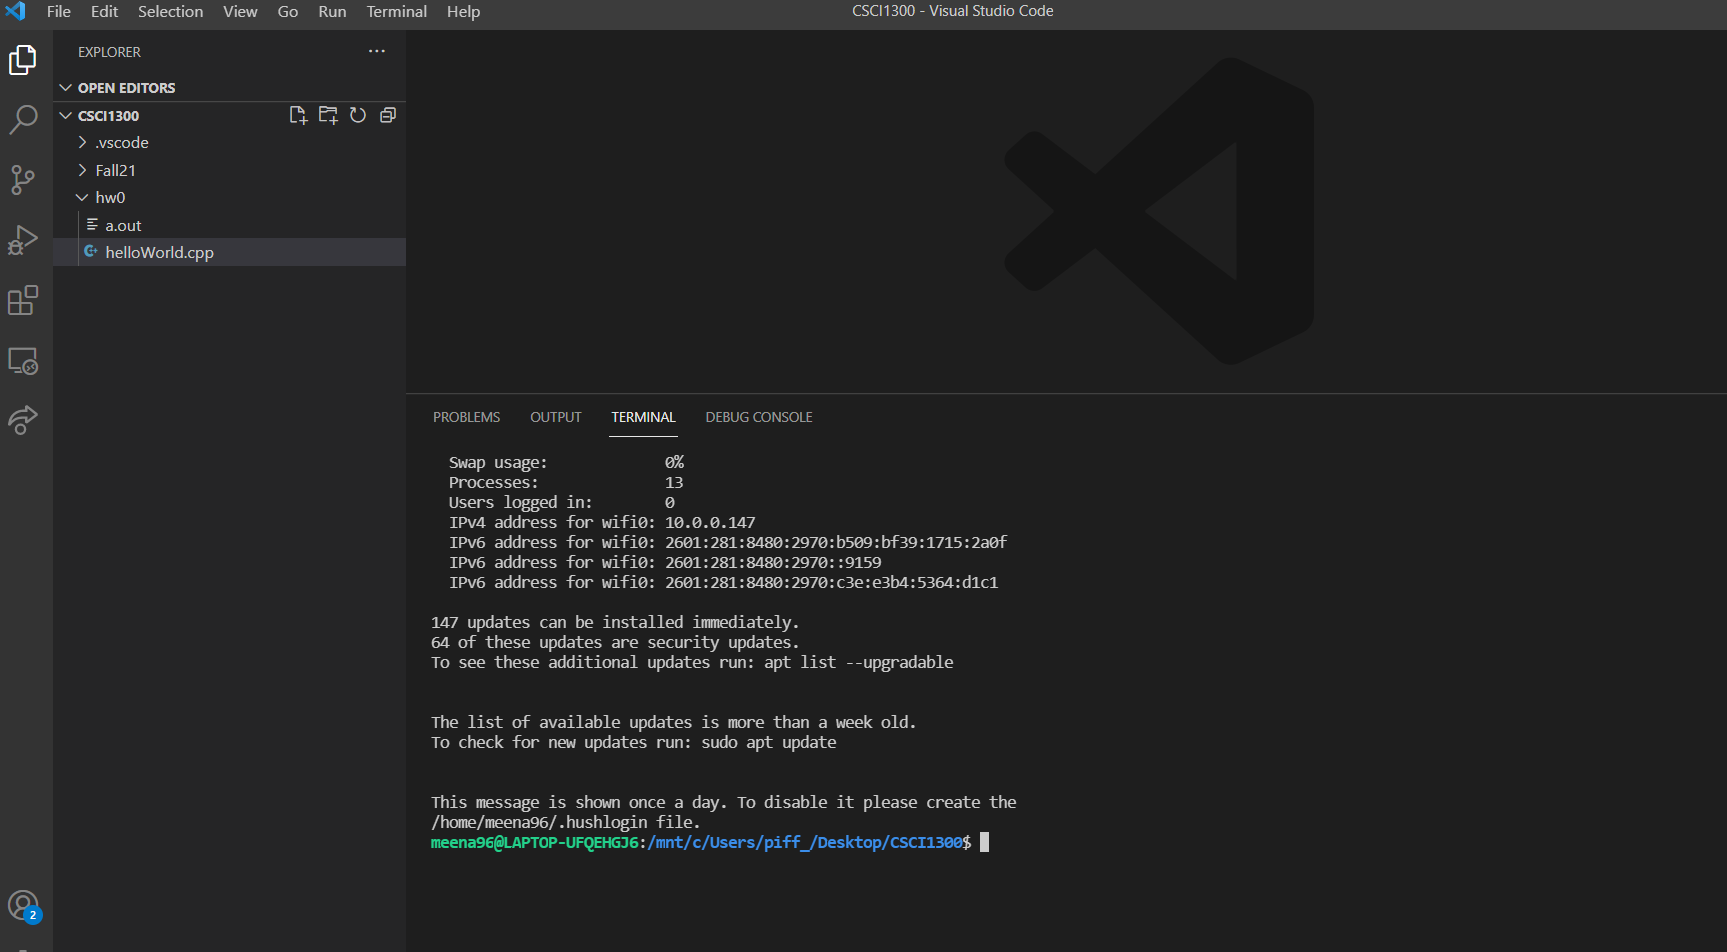
\includegraphics[width=\textwidth]{images/learn_terminal_4.png}

You will see your name and your device name on the terminal tab. Note that this can look different depending on your OS. The general anatomy of a terminal window is as follows:

\begin{enumerate}
    \item Everything before the : tells you the username and the device name you’re logged in
    \item Everything between the : and \$ is your current directory (think of a directory as the folder you’re in). Note that you do not need to be in the same directory as the screenshots shown above. Yours will depend on your computer. Mac/Linux and Windows will look different, but both will state the current directory (or ``folder") that you are in.
    \item \$ represents the end of the prompt, after which you can enter a command.
\end{enumerate}


File browsing using the terminal is like using Windows explorer/Finder or clicking on folders and navigating to different folders on your machine.

In the terminal, instead of clicking on folders we use text commands to tell the computer what we want. If we want to go to a folder where we saved our last homework, we can type the commands to navigate to that folder and display its contents.

You can read file and folder locations by their ``pathname", which is just a list of directories needed to get to your current location. Note: ``folder" and ``directory" mean the same thing, but most computer science texts will use the word ``directory". There are two different ways of expressing pathnames that you will come across; one is a constant pathname, which describes how to access a location from anywhere. A second one is a relative path name, which tells you how to get to a location from your current location. If you are already in a folder. You may see these pathnames have something like ``..", which tells the computer to go back a directory from the current location, but otherwise the style of these pathnames will look similar. 

You will need to learn the basic text commands to navigate your computer system using the terminal. Important commands to learn include how to change which folder you are in, how to see the contents of your current folder, and more. Here is a list of commands and their meanings:

\begin{table}[H]
    \begin{tabular}{p{2.5in}|p{4.0in}}
        \mintinline{bash}{ls} &  list directory contents. Note, this a lowercase l, not an uppercase ``i". This will `list' everything in the current directory. \\
        \mintinline{bash}{cd [location]} & change directory, taking you to the specified [location]. \\
        \mintinline{bash}{mkdir [name]} & make directory, which will make a new directory inside of your current location using the provided [name]. \\
        \mintinline{bash}{cp [from here] [to here]} & copy a specified file from the first specified location to the second specified location. \\
        \mintinline{bash}{mv [from here] [to here]} & move a specified file from the first specified location to the second specified location. \\
        \mintinline{bash}{zip [zip file] [listed files]} & Zip all listed files into a new zip file called [zip file]. \\
        \mintinline{bash}{rm [file name]} & permanently delete the file called [file name].
    \end{tabular}
\end{table}

Note, the square brackets are not part of the command but only to illustrate where you should insert some other text.

Finally, you will need to know how to compile code from your terminal. Let us say that we have some code in a file called ``helloWorld.cpp". In order to compile this program, we would have to navigate to the directory containing this file. Once there, you will enter the command:

\begin{minted}{bash}
        g++ -std=c++17 helloWorld.cpp 
\end{minted}

\mintinline{bash}{g++} is the compiler program.

\mintinline{bash}{-std=c++17} is the version of C++ we want to use.

\mintinline{bash}{helloWorld.cpp} is the file we wish to compile.

This command creates a file named a.out which is the compiled version of the code in helloWorld.cpp, which can be executed. You can run this compiled code using the following command:

\begin{minted}{bash}
        ./a.out
\end{minted}

Pro Tips:
\begin{itemize}
    \item Tab Complete: if you're typing something in the command line that’s very long, but unique, you can hit tab when you're partially through and it will try to fill in the rest (kind of like autocomplete). If it doesn't, and you press tab twice, it tells you everything it has as options.
    \item Command history browsing: if you have typed a command and want to repeat it, just press the up arrow. It will bring up your last executed command. Pressing up again will go to the one before. Pressing down will go forward in time through the list.
\end{itemize}

\subsection{Anatomy of a C++ Program}

You will need a couple of components for the computer to be able to understand how to translate code that you can read into something it can actually do. 

Here is a snapshot of a basic ``Hello World" program from the course textbook,  Brief C++: Late Objects, Enhanced eText. 

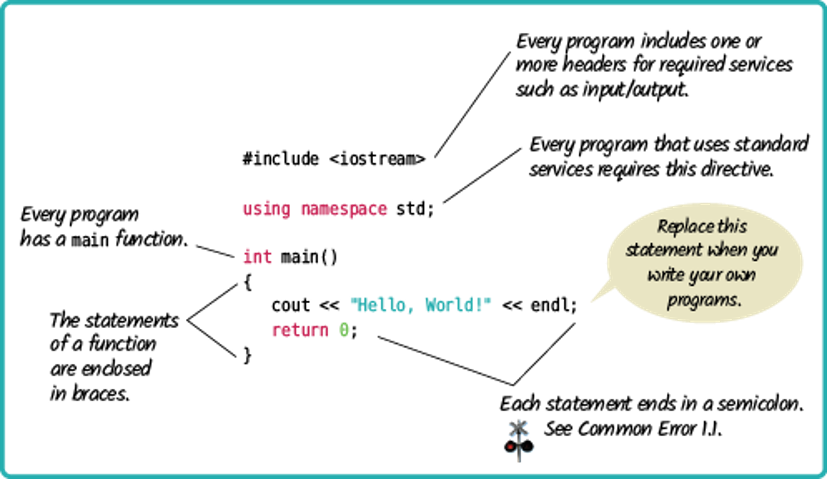
\includegraphics[width=\textwidth]{images/hello_world_16.png}

\subsection{Variables and Operators}
This week we learned about variables and basic arithmetic operators in computer science. 

Variables in computer science are similar to variables you have seen in other math and science courses. A \textbf{variable} is a value that can change, depending on conditions or on information passed to the program.

A computer stores variables differently depending on the type of information they are meant to contain, so we must declare the type of variable. This table will tell you the names of different types of variables in C++:

\begin{table}[H]
    \centering
    \begin{tabular}{c|c|c|c}\hline
         Type of variable & Declaration in C++ & Size & Description \\\hline
         Integer & int & 2 or 4 bytes & a number that has no decimal value \\
         Float & float & 4 bytes & a number that has short decimal values \\
         Double & double & 8 bytes & a number that can have longer decimals \\
         Character & char & 1 byte & stores a single letter/character using ASCII values \\
         Boolean & bool & 1 byte & stores either True or False 
    \end{tabular}
\end{table}

In order to create and use a variable, you must declare it using the appropriate declaration from the above table and then give it a name. You may also provide it an initial value, but this is not required to create a variable. Some examples include:

\begin{example}
Here is an example of declaring variables:
\begin{minted}{c++}
int myNumber = 0;
double myDecimal = 3.1415;
char myEmptyChar;
\end{minted}
\end{example}

After declaring variables, you can access them without repeating their data type. You can also perform basic operations, including the ones listed in this table:

\begin{table}[H]
    \centering
    \begin{tabular}{c|c|c}\hline
        Operator & Description & Example \\ \hline
        \mintinline{c++}{+}	& Adds together two values & \mintinline{c++}{x + y}\\
        \mintinline{c++}{+=} & Adds to itself and stores the new value& \mintinline{c++}{x += y}\\
        \mintinline{c++}{-} & Subtracts one value from another & \mintinline{c++}{x - y} \\
        \mintinline{c++}{*} &	Multiplies two values & \mintinline{c++}{x * y} \\
        \mintinline{c++}{/} & Divides one value by another & \mintinline{c++}{x / y} \\
        \mintinline{c++}{%} & Modulus; this returns the division remainder & \mintinline{c++}{x % y} \\
        \mintinline{c++}{++} & Increment; this increases the value of a variable by 1 & \mintinline{c++}{++x} \\
        \mintinline{c++}{--} & Decrement; this decreases the value of a variable by 1 & \mintinline{c++}{--x}
    \end{tabular}
\end{table}

\begin{example}
Here is an example of declaring variables and using operators:
\begin{minted}{c++}
    int myNumber = 4;
    int mySecondNumber = 5;
    int mySum = myNumber+mySecondNumber;
    int myThirdNumber = 6;
    mySum = mySum + myThirdNumber;
    int myFourthNumber = 7;
    mySum += myFourthNumber;
\end{minted}

By the end of this code, the variable \mintinline{c++}{mySum} would contain 4+5+6+7, or 22. 
\end{example}

\subsection{Terminal Input and Output}

It is important to be able to take input from the user or to print output to the terminal as your program runs. You can do this using \mintinline{c++}{cin} and \mintinline{c++}{cout} for input and output, respectively. 

The Hello World program you have seen provides an example of using \mintinline{c++}{cout} to display output.

\begin{example}
Hello World for C++:
\begin{minted}{c++}
    #include <iostream>

    using namespace std;

    int main() {
        cout << "Hello, world!" << endl;
        
        return 0;
    }
\end{minted}

\end{example}

You can similarly ask the user for a particular value and store that value in a variable using \mintinline{c++}{cin}:

\begin{example}
An example of collecting user input to sum two integer variables and then printing their sum
\begin{minted}{c++}
    #include <iostream>

    using namespace std;

    int main() {
        int firstNum;
        int secondNum;
        cout << "Please provide one number:" << endl;
        cin >> firstNum;
        cout << "Please provide a second number:" << endl;
        cin >> secondNum;
        cout << "The sum of these two numbers is " << firstNum + secondNum << endl;

        return 0;
    }
\end{minted}

\end{example}

\subsection{Pseudocode and Algorithms}

Pseudocode is used to develop algorithms. An algorithm is a procedure for solving a problem.

An algorithm describes actions to be executed and the order in which those actions are to be executed. In other words, an algorithm is merely the sequence of steps taken to solve a problem; like a recipe. An algorithm is not computer code. Algorithms are just the instructions which provide a clear path for you to write the computer code.

\begin{example}
    An algorithm for adding two numbers together:

Step 1: Start

Step 2: Declare variables num1, num2, and sum.

Step 3: Read values num1 and num2.

Step 4: Add num1 and num2 and assign the result to sum.

Step 5: Display sum

Step 6: Stop
\end{example}

The main difference between an algorithm and pseudocode is that an algorithm is a step by step procedure to solve a given problem while pseudocode is a method of writing an algorithm. In other words, an algorithm is how to solve a problem while pseudocode is how to implement that solution. 

\begin{table}[H]
    \centering
    \begin{tabular}{p{3 in}|p{3 in}} \hline 
    Algorithm 	& Pseudocode \\ \hline
An unambiguous specification of how to solve a problem. & An informal high-level description of the operating principle of a computer program or other algorithm. \\ \hline
Helps to simplify and understand the problem. & A method of developing an algorithm. \\\hline
    \end{tabular}
\end{table}

Pseudocode is informal language that helps programmers develop algorithms (or recipes). Although there are no hard and fast rules for pseudocode, there are some suggestions to help make pseudocode more understandable and easy to read.

For instance, consider indenting all statements showing a ``dependency”, like statements that use: While, do, for, if.

Several keywords are often used to indicate common input, output, and processing operations.

\begin{table}[H]
    \centering
    \begin{tabular}{c|c}
    Input:	& READ, OBTAIN, GET \\
    Output:	& PRINT, DISPLAY, SHOW \\
    Compute: & COMPUTE, CALCULATE, DETERMINE \\
    Initialize:	& SET, INITIALIZE \\
    Add one: & INCREMENT, BUMP \\
    \end{tabular}
\end{table}

For looping and selection, the keywords that you might consider writing include:
\begin{itemize}
    \item Do While...
    \item Do Until...
    \item Case...
    \item If… then...
    \item Call ... with (parameters)
    \item Call
    \item Return ....
    \item Return
    \item When
\end{itemize}

Try to indicate the end of loops and iteration by using scope terminators.
For instance use if… (statements) ... endif.

Other words you may find useful while writing pseudocode include: Generate, Compute, Process, set, reset, increment, compute, calculate, add, sum, multiply, subtract, divide, print, display, input, output, edit, test, etc.

Be sure to indent if the indentation fosters understanding. Being clear is the purpose of pseudocode, and a very desirable goal to strive for.

Here are some examples of pseudocode:

\begin{example} Will a grade pass?
\begin{minted}{c++}
If students grade is higher than or equal to 60
	Then Print, "Passed"
else
	Print, "Failed"
\end{minted}
    
\end{example}

\begin{example} How do you find the area of a rectangle?
\begin{minted}{c++}
Read the length of the rectangle
Read the width of the rectangle
Compute the area of the rectangle as length times width.
\end{minted}
    
\end{example}

You should write pseudocode whenever you are addressing problems in computer science. This allows you space to determine how to solve a problem without worrying about syntax and formatting, instead of having to figure out everything all at once. 

\section{Warm Up}
You will need to install and become familiar with the software we will be using this semester. Follow the appropriate installation guides in Appendix A for your particular computer (Windows or Mac) to install VS Code. 

Once you have installed your software you will need to open VS Code and open the terminal. You will need VS Code and a working terminal to complete the recitation this week. Take a screenshot and submit it on Canvas for this week's Warm Up assignment. 

\section{Recitation}

\subsection{Hello World}

The ``Hello, World!" program is one of the simplest programs in a programming language, and it is often used to illustrate the basic syntax of a programming language. We will need to first create a folder to store our program file in and then create the file to write the program.

First, open VS Code. You can make a new folder by clicking this button: 

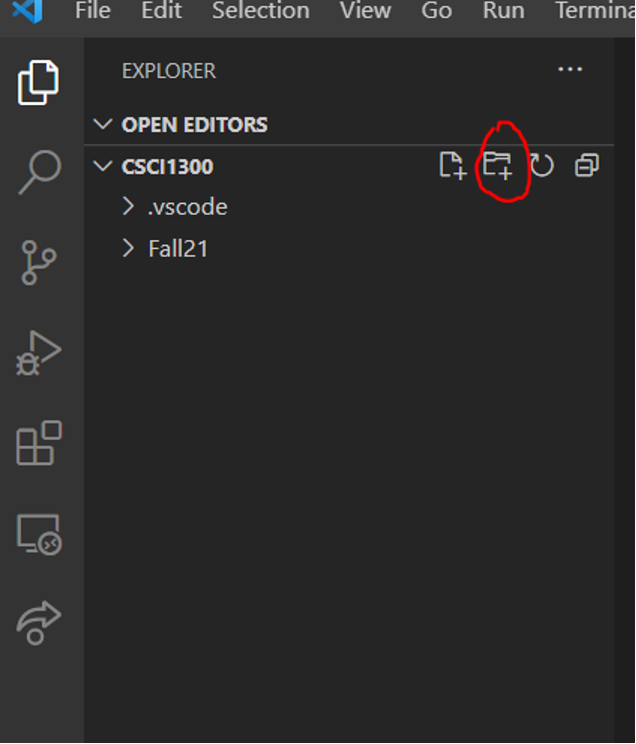
\includegraphics[width=7cm]{images/hello_world_2.png}

Name the folder something intuitive, like ``Week\_1", ``Recitation\_1", or similar. Once you have your folder you will need to create a file within it, which you can do with the toolbar across the top:

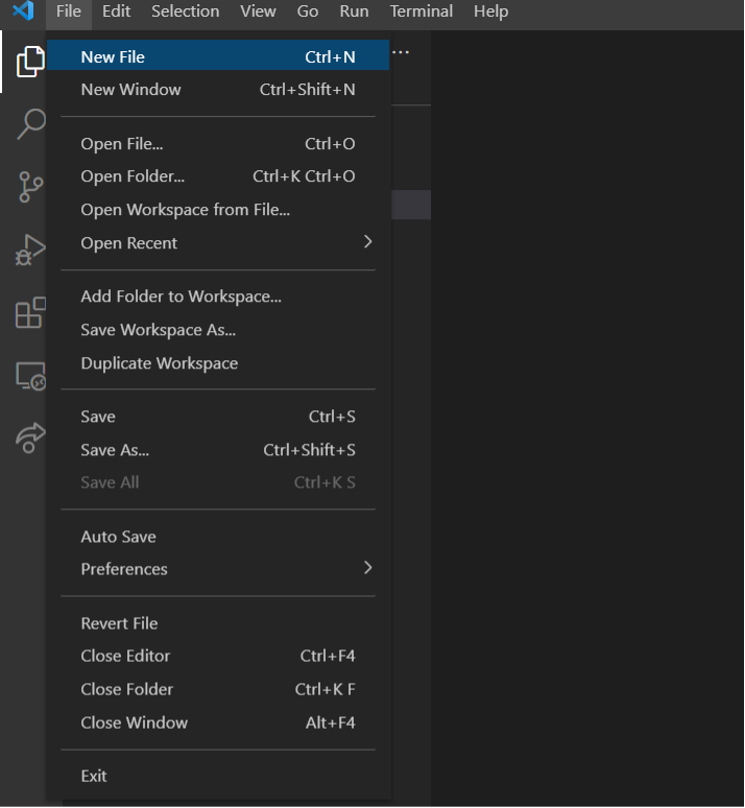
\includegraphics[width=7cm]{images/hello_world_4.png}

You should name your file \mintinline{c++}{helloWorld.cpp} -- this file name structure is important. Files of uncompiled C++ code should end with \mintinline{c++}{.cpp}, and the usage of a capital letter at the beginning of each word makes it legible even without spaces or punctuation. This style of writing names is often called ``camel case". 

Type the following code into your file:

\begin{minted}{c++}
    #include <iostream>

    int main() {
        std::cout << "Hello, world!" << std::endl;
    }
\end{minted}

Save your file.  A quick shortcut to save is Cmd + S (In Mac) or Ctrl + S (in Windows). Now you will need to compile and run your program. You can review the background information to see how to do this. Once you have completed this and successfully run your program, take a screenshot of your VS Code window including both the file and the terminal. 

Now, let us explore this program a little more. Add a statement to use the standard namespace. Insert \mintinline{c++}{using namespace std;} at the beginning of the code, then we can remove the \mintinline{c++}{std::} prefixes. Your new code should look like this:

\begin{minted}{c++}
    #include <iostream>

    using namespace std;
    
    int main() {
        cout << "Hello, world!" << endl;
    }
\end{minted}

Run the program again using the steps above. Take an additional screenshot.

Let’s modify the file to print ``Hello world! Hello CSCI 1300”. The text inside of the quotation marks is printed as it is. It’s case sensitive too! To see the updated output, compile and run again.

\begin{minted}{c++}
    #include <iostream>

    using namespace std;
    
    int main() {
        cout << "Hello, world! Hello CSCI 1300" << endl;
    }
\end{minted}

Once again, take a screenshot. For this section you should have three screenshots for the different Hello World programs; you will need to submit this on Canvas. 

\subsection{Variables}

\begin{multipart}
    What is a variable?
\end{multipart}

\vspace{2cm}

\begin{multipart}
    Consider a variable tracking changing cost of an item on Ebay. What would be a good name for this variable?
\end{multipart}

\vspace{1.5cm}

\begin{multipart}
    Consider a variable that represents the roll of a 6-sided die. What possible values could this variable hold? 
\end{multipart}

\vspace{1.5cm}

\begin{multipart}
    Consider a variable that tracks the temperature outside. What data type should you use? Are there multiple types that would work?
\end{multipart}

\vspace{1.5cm}

\subsection{Converting Seconds to Days:Hours:Minutes:Seconds}
A day has 86,400 seconds ($24 \times 60 \times 60$). Given a number of seconds in the range of 0 to 1,000,000 seconds, your program should print the time as days, hours, minutes, and seconds for a 24 hour clock. For example, 70,000 seconds is 0 days, 19 hours, 26 minutes, and 40 seconds. Your program should accept user input for the number of seconds to convert and then use that number in your calculations. Format your output as follows: 

\mintinline{c++}{The time is W days, X hours, Y minutes, and Z seconds.}

\begin{multipart}
    Explicitly list the variables you will need and their data types. 
\end{multipart}

\vspace{3cm}

\begin{multipart}
    What arithmetic operators will be most useful for this problem?
\end{multipart}

\vspace{2cm}

\section{Homework}
\subsection{Hello, Name!}
You have recently learned how to accept user input and store it in a variable. Write a program where you ask the user for their name in the terminal, and then print \mintinline{c++}{Hello, [name]!} in the terminal. You may find it helpful to start with the Hello World program from recitation. 

A few example runs are shown below. In these examples, red text represents user-provided text (or text you would have to type in the terminal while running the program). 

\begin{sample}
What is your name?

\textcolor{red}{Mike}

Hello, Mike!
\end{sample}

\begin{sample}
What is your name?

\textcolor{red}{samantha}

Hello, samantha!
\end{sample}

\subsection{Volume to Ounces}

While shopping over the weekend for almond milk, you discover that all the almond milk cartons have square bases and varying heights. Write an algorithm which takes user inputs for the side length of the square base of the carton in inches and the height of the carton in inches and outputs how many ounces a carton holds. You can use the following formula to convert cubic inches to ounces:

$$1 in^3 = 0.554 oz$$

Hint: you should calculate cubic inches from the carton's dimensions before calculating ounces.

\begin{sample}
What is the side length of the base of the carton in inches?

\textcolor{red}{4}

What is the height of the carton in inches?

\textcolor{red}{5}

The carton has a volume of 44.33 oz
\end{sample}

You will need to submit pseudocode for this solution -- NOT code. You do not have to have a coded or tested solution for this, only a set of step-by-step instructions for how someone else might write the code.  

\subsection{Converting Seconds to Days:Hours:Minutes:Seconds}
You will need to code the question discussed in Recitation section 3.3. The question is:

A day has 86,400 seconds ($24 \times 60 \times 60$). Given a number of seconds in the range of 0 to 1,000,000 seconds, your program should print the time as days, hours, minutes, and seconds for a 24 hour clock. For example, 70,000 seconds is 0 days, 19 hours, 26 minutes, and 40 seconds. Your program should accept user input for the number of seconds to convert and then use that number in your calculations. Format your output as follows: 

\mintinline{c++}{The time is W days, X hours, Y minutes, and Z seconds.}

You should start by writing the algorithm on paper, using the variables and arithmetic operators you identified in recitation. You will then need to write the code for this question and submit this via Canvas. 

Here are a few example runs:

\begin{sample}
    How many seconds (between 0 to 1,000,000) would you like to convert to Days, Hours, Minutes, and Seconds?

    \textcolor{red}{70000}

    The time is 0 days, 19 hours, 26 minutes, and 40 seconds.
\end{sample}

\begin{sample}
    How many seconds (between 0 to 1,000,000) would you like to convert to Days, Hours, Minutes, and Seconds?

    \textcolor{red}{409176}

    The time is 4 days, 17 hours, 39 minutes, and 36 seconds.
\end{sample}


\subsection{Identify and Correct the Errors}
There are several snippets of code below where there is one error. You will need to identify and correct the error so that the code compiles. This code is also available directly in CodeRunner. 

\begin{multipart}
Spot the error:


    \begin{minted}{c++}
#include <iostream> 
using namespace std;
						
int Main()
{
	cout << "Hello, World!" << endl;
	return 0; 
}
    \end{minted}
\end{multipart}

\begin{multipart}
Spot the error:


    \begin{minted}{c++}
#include <iostream> 
using namespace std;
						
int main 
{
	cout << "Hello, World!" << endl;
	return 0; 
}
    \end{minted}
\end{multipart}

\begin{multipart}
Spot the error:


    \begin{minted}{c++}
#include <iostream> 
using namespace std;
						
int main() 
{
	cout << "Hello, World! << endl;
	return 0; 
} 
    \end{minted}
\end{multipart}

\begin{multipart}
Spot the error:


    \begin{minted}{c++}
#include <IOstream> 
using namespace std;
						
int main() 
{
	cout << "Hello, World!" << endl
	return 0; 
} 
    \end{minted}
\end{multipart}

\begin{multipart}
Spot the error:


    \begin{minted}{c++}
#include <iostream> 
using namespace;
						
int main() 
{
	cout << "Hello, World!" < endl; 
}
    \end{minted}
\end{multipart}
